\documentclass[conference]{IEEEtran}
\IEEEoverridecommandlockouts
% The preceding line is only needed to identify funding in the first footnote. If that is unneeded, please comment it out.
\usepackage{cite}
\usepackage{amsmath,amssymb,amsfonts}
\usepackage{algorithmic}
\usepackage{graphicx}
\usepackage{textcompthe_annotated_transformer}
\usepackage{xcolor}
\usepackage[backend=biber,
            sorting=none,   % Keine Sortierung
            doi=true,       % DOI anzeigen
            isbn=true,     % ISBN nicht anzeigen
            url=true,       % URLs anzeigen
            maxnames=6,     % Ab 6 Autoren et al. verwenden
            minnames=1,     % und nur den ersten Autor angeben
            style=numeric-comp,]{biblatex}
\addbibresource{literatur.bib}

\def\BibTeX{{\rm B\kern-.05em{\sc i\kern-.025em b}\kern-.08em
    T\kern-.1667em\lower.7ex\hbox{E}\kern-.125emX}}
\begin{document}

\title{Transformer gibt es nicht nur im Kino}


\author{\IEEEauthorblockN{Jonathan Arns}
\IEEEauthorblockA{\textit{Hochschule Mannheim} \\
Fakultät für Informatik\\
Paul-Wittsack-Str. 10\\
68163 Mannheim\\
jonathan.arns@stud.hs-mannheim.de}
}

\maketitle

%%%%%%%%%%%%%%%%%%%%%%%%%%%%%%%%% Document beginning %%%%%%%%%%%%%%%%%%%%%%%%%%%%%%%%%%%%%%

\begin{abstract}
abstract
\end{abstract}


\section{Einleitung}
Natural Language Processing (NLP), die Verarbeitung Menschlicher Sprache, ist ein Anwendungbereich für Machine Learning, der bereits erheblich von deep neural networks (DNN) profitiert hat. Die zwei dominanten Arten von DNN Architekturen dabei waren lange Zeit recurrent neural networks (RNN) und convolutional neural networks (CNN). \cite{comparative_study_cnn_rnn}

2017 stellten Vaswani et al. \cite{attention_is_all_you_need} mit dem Transformer eine neue DNN Architektur vor, die seitdem unter Anderem große Aufmerksamkeit durch die erfolgreiche Verwendung in OpenAIs GPT-2 und GPT-3 Modellen erlangte.

\section{Sequence to Sequence Learning}
Traditionell waren DNNs trotz ihrer hohen Flexibilität und Effektivität für viele Aufgaben beschränkt auf Probleme, deren Eingaben und Ausgaben sich sinvoll in Vektoren mit fester Länge codieren lassen, da neuronale Netze generell eine feste Anzahl an Eingabe- und Ausgabeneuronen haben. Das ist zwar für viele Klassifizierungsprobleme und in der Bildverarbeitung kein Problem, sehr wohl aber für beispielsweise NLP, da die Länge von Texten im Vorfeld nicht immer bekannt ist. \cite{sequence_to_sequence}

Dieses Problem wird mittels Sequence to Sequence (Seq2Seq) Learning gelöst, mit dessen Hilfe beliebig lange Sequenzen von Elementen als Eingabe in vollkommen andere Sequenzen, anderer Länge und aus anderen Elementen, transformiert werden können. \cite{sequence_to_sequence}

Die meisten Seq2Seq Modelle bestehen aus einem Encoder und einem Decoder \cite{attention_is_all_you_need}. Der Encoder codiert die Eingabe Sequenz in einer höher-dimensionale Vektorrepräsentation, die dann vom Decoder in eine Ausgabe Sequenz umgewandelt wird. Die Encoder und Decoder selbst sind in der Regel RNNs, beispielsweise mit der LSTM Architektur.



\section{Attention}
Attention ist der wichtigste Mechanismus des Transformers. Attention erlaubt dem Transformer beispielsweise, Sätze nicht nur Wort für Wort zu übersetzen, sondern Zusammenhänge zu erkennen und grammatikalisch korrekte Sätze zu bilden. Abstrakt ist eine Attention Funktion eine Abbildung von einer Query und einer Menge von Key-Value Paaren zu einer Ausgabe. In einem Übersetzungskontext könnte das Wort, welches gerade übersetzt werden soll, die Query sein und alle Wörter in dem zu übersetzenden Satz die Keys und Values. Das Ergebnis signalisiert dann, welche Wörter bei der Übersetzung der Query zusätzlich besonders in betracht gezogen werden. Diese spezielle Konstellation, in der die Query, Keys und Values aus der gleichen Sequenz stammen, nennt sich Self-Attention. Diese kommt auch im Transformer zum Einsatz und ist beispielhaft in Abb. \ref{fig:4} visualisiert.
\begin{figure}[htbp]
\centerline{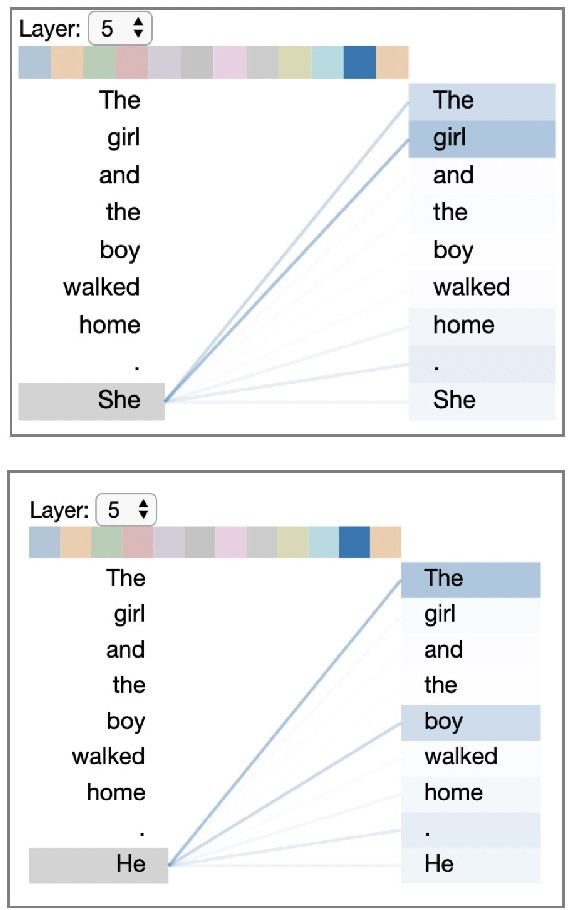
\includegraphics{img/attention_visualized.png}}
\caption{Visualisierung von Self-Attention in GPT-2. Verbindungen von der Query (grau hinterlegt) zu den Keys zeigen Attention, dunklere Verbindungen sind höher gewichtet. Hier ist sichtbar, wie mittels Attention Referenzen auf frühere Wörter erkannt werden können. \cite{visualization_of_attention}}
\label{fig:4}
\end{figure}

\subsection{Scaled dotproduct attention}
Es gibt grundlegend zwei verschiedene Attention Funktionen, additive Attention und dot-product Attention. Der Transformer verwendet dot-product Attention, da diese trotz gleicher theoretischer Komplexität in der Praxis aufgrund von hoch optimiertem Matix-Multiplikations Code deutlich schneller ist. Abb. \ref{fig:2} zeigt den Aufbau eines scaled dot-product attention Moduls im Transformer. Die Berechnung der Attention Matrix erfolgt mit folgender Formel:
\begin{equation} \label{eq:attention}
    Attention(Q,K,V) = softmax(\frac{QK^T}{\sqrt{d_K}})V
\end{equation}
Dabei ist $Q$ die Matrix der Query Vektoren, $K$ die Matrix der Key Vektoren und $V$ die Matrix der Value Vektoren. $Q$ ist entgegen der Intuition eine Matrix, da die Attention in der Praxis mittels Matrizenoperationen für mehrere Queries auf einmal berechnet wird.

Softmax, die normalisierte Exponentialfunktion, normalisiert alle Elemente eines Vektors auf Werte zwischen $0$ und $1$, so dass die Summe aller Werte $1$ ergibt. Da die Exponentialfunktion verwendet wird, nähert sich das größte Element des Vektors $1$ an, während sich, außer in sehr knappen Fällen, alle anderen Elemente $0$ annähern. Sei $x$ ein Vektor mit den Elementen $x_1 ... x_n$, dann ist Softmax wie folgt definiert. \cite{softmax_to_softassign}
\begin{equation} \label{eq:softmax}
    Softmax(x)_j = \frac{e^{\beta x_j}}{\sum_{i = 1}^{n} e^{\beta x_i}}, \beta \in \mathbb{R} \land \beta > 0
\end{equation}
Da die Softmax Funktion in der Praxis nicht gut mit sehr großen Werten skaliert, werden die Scores mit der Wurzel der Dimension der Keys $\sqrt{d_k}$ skaliert, bevor Softmax berechnet wird. \cite{attention_is_all_you_need}

\begin{figure}[htbp]
\centerline{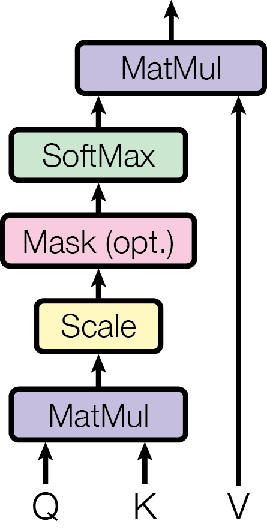
\includegraphics{img/scaled_dotproduct_attention.png}}
\caption{Für die Berechnung der Scaled Dotproduct-Attention werden die Matrizen $Q$, $K$ und $V$ benötigt. Die Queries $Q$ und die Keys $K$ haben die Dimension $d_k$, die Values $V$ haben die Dimension $d_v$. Um die Attention zu berechnen, wird mittels Matrixmultiplikation der Queries mit den transponierten Keys pro Query Vektor ein Score für jeden Key gebildet. Diese Scores werden mit $\sqrt{d_k}$ skaliert und mit einer Softmax Funktion pro Query zu Gewichten für die Values normalisiert. Um die Attention Matrix zu erhalten werden die Values mit den ermittelten Gewichten multipliziert. Vor der Berechnung der Softmax Funktion werden optional Werte maskiert, die noch unerlaubte Verbindungen darstellen. Zu maskierende Werte werden auf $-\infty$ gesetzt. \cite{attention_is_all_you_need}}
\label{fig:2}
\end{figure}

% Sei die Eingabe eine Sequenz aus zwei Elementen, die in den Vektoren $x_1$ und $x_2$ ... codiert sind.
% Jeder Eingabe Vektor wird mit den Matrizen $W^Q$, $W^K$ und $W^V$ multipliziert, um die Query-Vektoren $q_1$ und $q_2$, die Key-Vektoren $k_1$ und $k_2$ und die Value-Vektoren $v_1$ und $v_2$ zu erzeugen. $W^Q$, $W^K$ und $W^V$ sind Gewicht-Matrizen, die zufällig initialisiert und beim Training des Modells erlernt werden.
% Im zweiten Schritt wird für jedes Element pro Query ein Score berechnet. Dazu wird jeweils das Skalarprodukt des Query-Vektors mit dem einzelnen Key-Vektor berechnet. Die Scores werden Skaliert, indem sie durch die Quadratwurzel der Dimension der Key-Vektoren $\sqrt{d_k}$ dividiert werden. Diese Skalierung wird verwendet, um die Performance der nachfolgenden Softmax Funktion bei sehr großen Eingaben zu verbessern. Aus den skalierten Scores werden mit der Softmax Funktion Gewichte für die Value-Vektoren berechnet. Softmax normalisiert die Eingaben auf Werte zwischen $0$ und $1$ so, dass ihre Summe $1$ ergibt. Die Value-Vektoren werden mit den berechneten Gewichten multipliziert, um das Ergebnis der Attention Funktion zu erhalten.


\subsection{Single-Head Attention}
Bei der Definition der dot-product Attention bis hier her fehlt noch ein essentieller Teil des Attention Mechanismus. Es fehlt jede Art von Parametern, die beim Training des Modells erlernt werden und die den Eingaben eine Gewichtung verleihen. Die Matrizen $Q$, $K$ und $V$, die die Attention Funktion als Eingaben erwartet, sind nicht einfach eine direkte Repräsentation der Eingaben des Modells, sondern gewichtete Projektionen von diesen, die zur Berechnung der Attention gebildet werden. Hierzu werden die Parameter Matrizen $W^Q$, $W^K$ und $W^V$ benötigt, mit denen die Eingaben einer Attention Schicht multipliziert werden. $W^Q$, $W^K$ und $W^V$ werden zufällig initialisiert und beim Training des Modells erlernt. In einem Single-Head Attention Modul haben die Projektionen die Dimension $d_{model}$, die der Dimension der codierten Eingaben des Modells entspricht. \cite{attention_is_all_you_need}

\subsection{Multi-Head Attention}
\begin{figure}[htbp]
\centerline{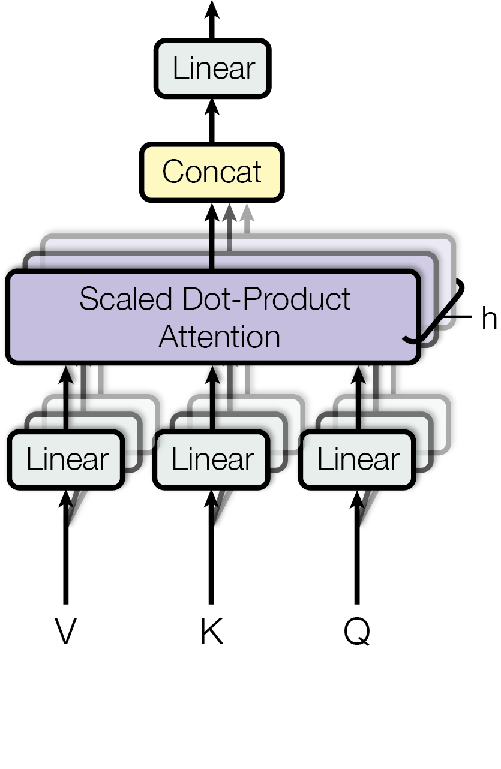
\includegraphics{img/multi_head_attention.png}}
\caption{Multi-Head Attention \cite{attention_is_all_you_need}}
\label{fig:3}
\end{figure}
Der Transformer verwendet anstatt Single-Head Attention Multi-Head Attention. Der Unterschied besteht darin, dass es mehrere Parameter Matrizen $W_1^Q$ ... $W_h^Q$, $W_1^K$ ... $W_h^K$ und $W_1^V$ ... $W_h^V$ gibt, mit denen die Eingaben linear projeziert werden. So werden $h$ so genannte Attention Heads gebildet. Die Projektionen haben anstatt $d_{model}$ die Dimensionen $d_k$, $d_k$ und $d_v$, wobei $d_k$ und $d_v$ kleiner sein können, als $d_{model}$. Für jede Projektion wird dann einzeln die Attention berechnet, die Ergebnisse werden concatiniert und mit einer weiteren Parameter Matrix $W^O$ in die $d_{model}$-dimensionale Ausgabe des Multi-Head Attention Moduls projeziert. Dieser Aufbau ist in Abb. \ref{fig:3} dargestellt und entspricht der Formel:
\begin{eqnarray} \label{eq:multi_head_attention}
    MultiHead(Q,K,V) = Concat(head_1,...,head_h)W^O \\
    \text{mit} \; head_i = Attention(QW_i^Q , KW_i^K , VW_i^V)
\end{eqnarray}
Wobei die Projektionen mit $W_i^Q \in \mathbb{R}^{d_{model} \times d_k}$, $W_i^K \in \mathbb{R}^{d_{model} \times d_k}$, $W_i^V \in \mathbb{R}^{d_{model} \times d_v}$ und $W^O \in \mathbb{R}^{hd_v \times d_{model}}$ definiert sind. \cite{attention_is_all_you_need}

Yin et al. \cite{attention_is_all_you_need} verwenden in ihrem Modell $h = 8$ und $d_k = d_v = \frac{d_{model}}{h}$, somit haben sie 8 kleinere Attention Heads bei ähnlichem Rechenaufwand im Vergleich zu einem $d_{model}$-dimensionalen Single-Head Attention Modul.

\subsection{Attention Beispiel}
% TODO


\section{Modell Architektur}
Fig. \ref{fig:1} zeigt die Architektur des Transformers. Der Transformer ist auto-regressiv, das bedeutet, dass jedes generierte Element der Ausgabe Sequenz ebenfalls als Eingabe Verwendet wird, um das nächste Element zu generieren \cite{attention_is_all_you_need}. Um eine vollständige Ausgabe zu erzeugen muss der Transformer also mehrfach ausgeführt werden.
% Im Folgenden wird weiter auf die wichtigsten Bestandteile der Transformer Architektur eingegangen.
\begin{figure}[htbp]
\centerline{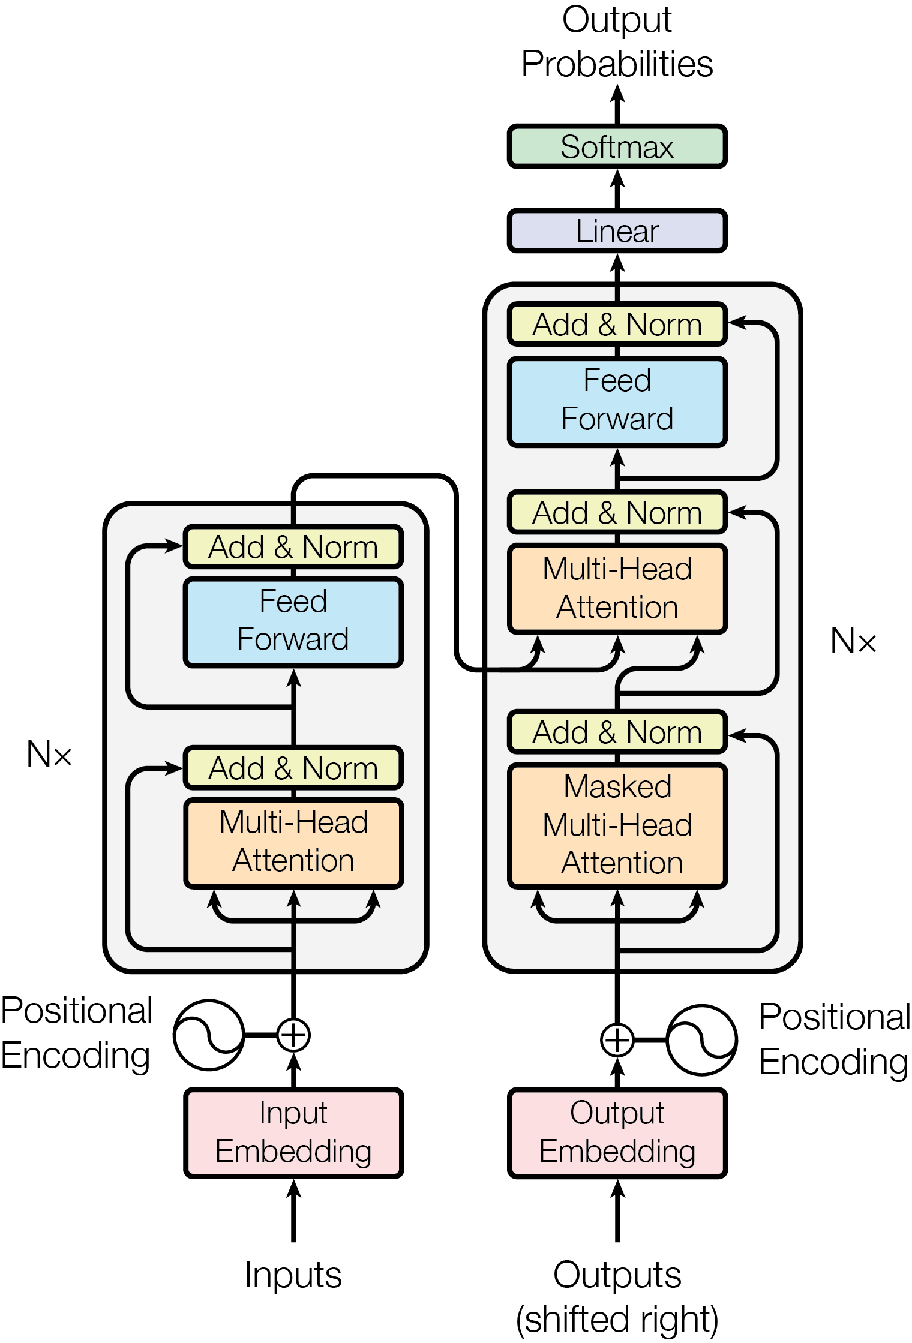
\includegraphics{img/figure1.png}}
\caption{Der Encoder (links) besteht aus einer Reihe von N identischen Schichten mit jeweils zwei Unterschichten. Die Eingaben einer Encoder Schicht fließen zuerst durch eine self-attention Schicht und dann durch ein feed-forward Netz. \\
Der Decoder (rechts) besteht auch aus einer Reihe von N identischen Schichten, jedoch mit jeweils drei Unterschichten. Die erste ist ebenfalls eine self-attention Schicht, deren Eingaben allerdings maskiert werden, um dem Modell keine Eingaben zu zeigen, die es nicht sehen sollte. Danach kommt eine Encoder-Decoder attention Schicht, die als Keys und Values die Ausgaben des Decoders und als Queries die Ausgaben der zuvor liegenden self-attention Schicht erhält. Zuletzt liegt wie beim Encoder ein feed-forward Netz. \\
Nach jeder Attention und feed-forward Schicht wird die Summe dessen Ausgaben und Eingaben zusammen normalisiert. Die normalisierten Werte dienen jeweils als Eingabe für die nächste Schicht. \\
Im NLP Anwendungen müssen die Eingaben für das Modell als erstes in Vektoren eingebettet werden. Da in Seq2Seq Modellen die Reihenfolge der Eingaben eine Rolle spielt, das Modell die Eingaben aber alle gemeinsam erhält, muss außerdem für jedes Element die Position in der Eingabe codiert werden. Der Transformer generiert für jedes Element einen Vektor, der dessen Position codiert, dazu stehen verschiedene Algorithmen, sowohl fix, als auch trainierbar, zur Verfügung. \\
Um ein Ergebnis zu erhalten, werden die Ausgaben des Decoders in einen Logit-Vektor transformiert und mit der Softmax Funktion normalisiert. Der erzeugte Vektor enthält für jedes Element des Ausgabealphabets die Wahrscheinlichkeit, dass es das nächste Element in der Ausgabe Sequenz ist. \cite{attention_is_all_you_need}}
\label{fig:1}
\end{figure}

\subsection{Anwendungen von Attention}
Der Transformer verwendet den Attention Mechanismus auf drei verschiedene Arten.
\subsubsection{Encoder Self-Attention}
In Self-Attention Schichten werden die gleichen Werte als Keys, Values und Queries verwendet. Durch die Self-Attention Schichten können für jedes Element im Encoder Abhängigkeiten zu jedem Element der Eingabe, beziehungsweise der Ausgabe der vorherigen Encoder Schicht, dargestellt werden.
\subsubsection{Decoder Self-Attention}
Durch die Self-Attention Schichten im Decoder können für jedes Element im Decoder ebenfalls Abhängigkeiten zu jedem Element der Ausgabe bis hin zum aktuellen Element dargestellt werden. Verbindungen zu Elementen nach dem jeweiligen Element sind nicht erlaubt, damit Ausgaben tatsächlich nur auf der Eingabe und bereits generierten Elementen basieren. Unerlaubte Verbindung werden durch eine Maskierung von Werten in der Attention Funktion verhindert.
\subsubsection{Encoder-Decoder Attention}
Die Keys und Values der Encoder-Decoder Attention Schichten im Decoder sind die Ausgaben des Encoders. Als Queries werden jeweils die Ausgaben der zuvor liegenden Self-Attention Schicht im Decoder verwendet. Damit können Abhängigkeiten von jedem Element im Decoder zu jedem Element der Encoder Ausgabe dargestellt werden. Hier besteht also die Schnittstelle vom Encoder zum Decoder und entsprechend die Beziehung zwischen den Eingabe und Ausgabe Sequenzen.

\subsection{Feed-Forward Netze}


\section{Training}
Die Modell Parameter werden zufällig initialisiert.


\section{Fazit}
Das ist ein Fazit



\printbibliography

\end{document}
